\subsection{Izbira zobnikov in jermenov}
\subsubsection{Vrtilna hitrost glavnega vretena}
Na stroju imamo motor z vrtilno hitrostjo 1410 \( \frac{vrt}{min} \)
V Tabeli \nameref{tabela_za_izbiro_hitrosti} lahko razberemo, da potrebujemo jermen na motorju
\( d_1 = \phi 107 \) in \( d_2 = \phi 191 \).
Na spodnji Sliki \ref{slika_prenosov} pa lahko vidimo shemo
zobniških in jermenskih prenosov.

\begin{figure}[H]
	\begin{center}
		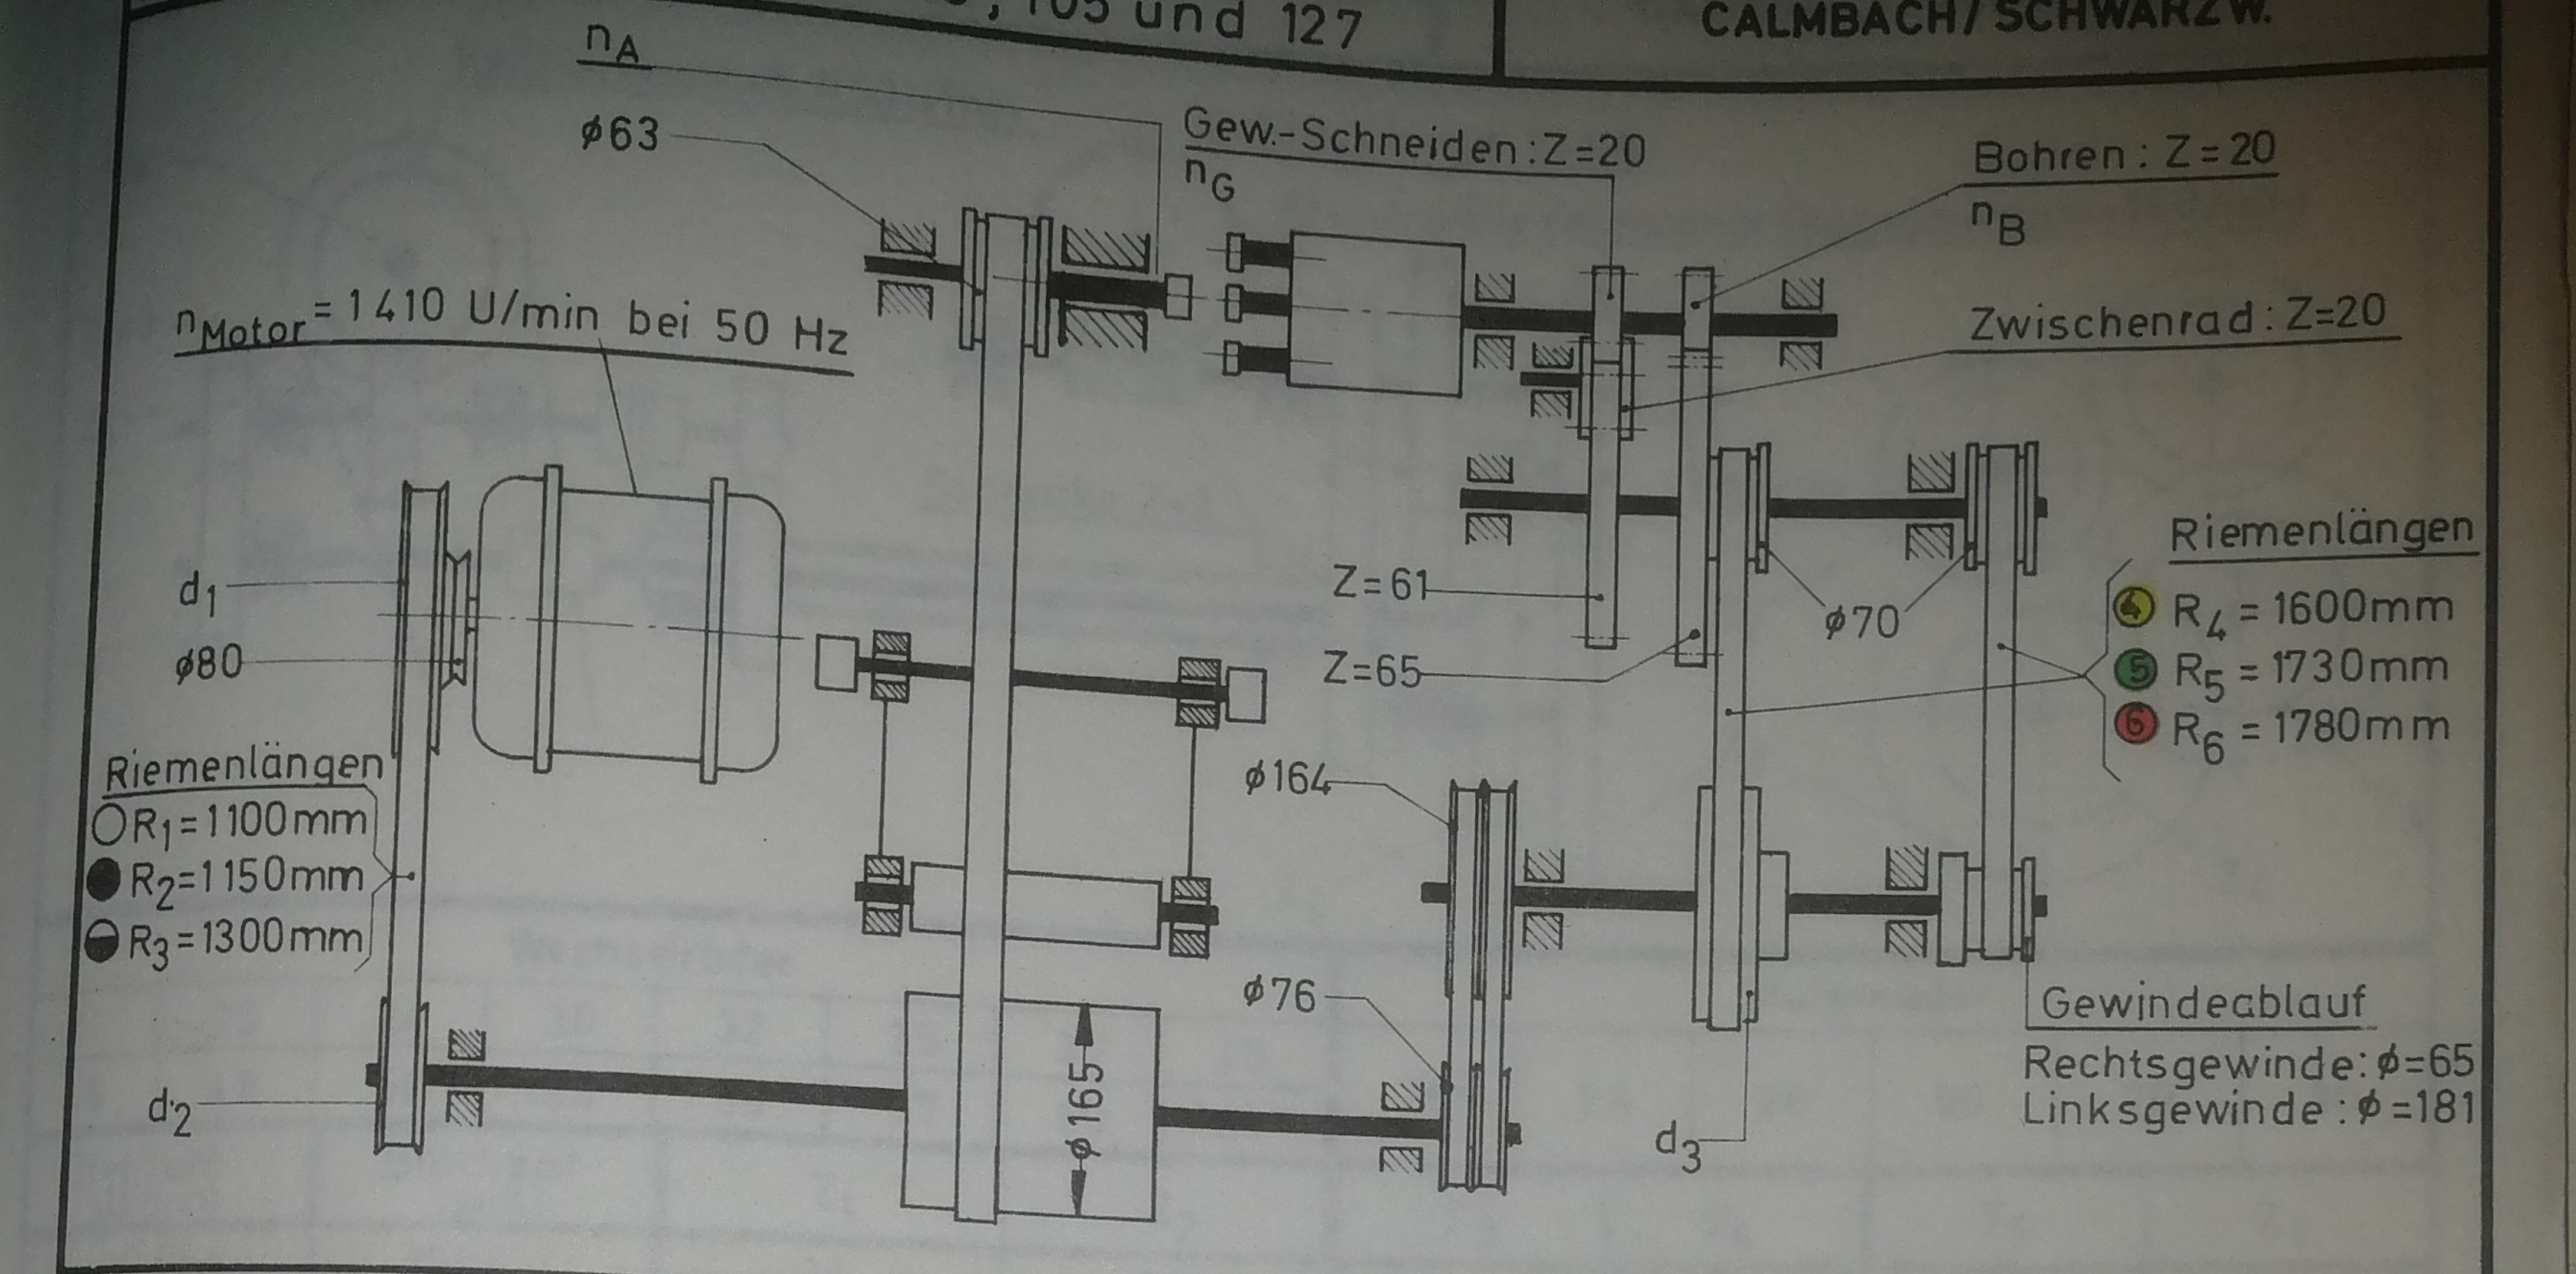
\includegraphics[width=\linewidth]{shema_prenosov_original.jpg}
		\caption{Slika sheme prenosov vrtilnih hitrosti
			\cite{gauthier}}
		\label{slika_prenosov}
	\end{center}
\end{figure}

Za boljšo preglednost sem zgornjo Sliko \ref{slika_prenosov}
prerisal in jo prikazal na spodnji Sliki \ref{skica_prenosov}

\begin{figure}[H]
	\begin{center}
		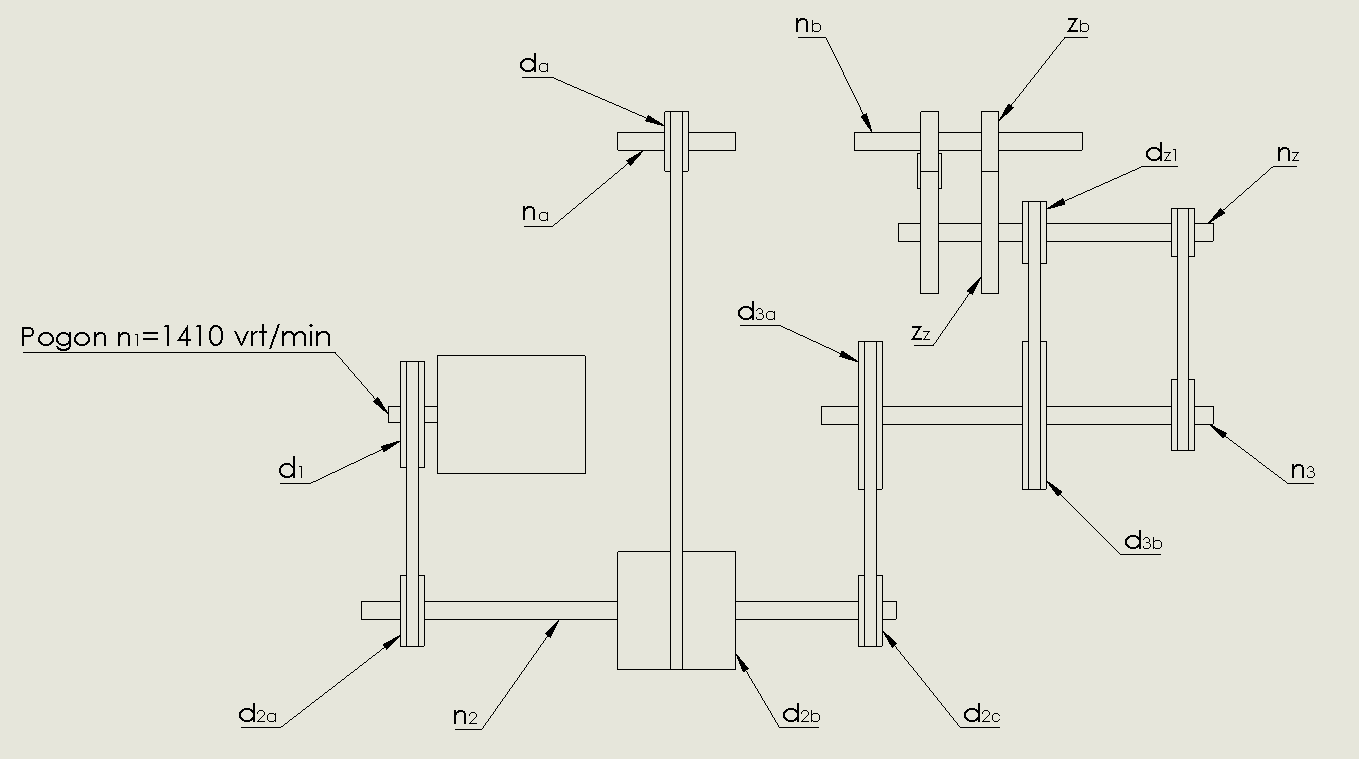
\includegraphics[width=\linewidth]{shema_prenosov_narisano.png}
		\caption{Prerisana shema prenosov vrtilnih hitrosti
			\cite{lasten}}
		\label{skica_prenosov}
	\end{center}
\end{figure}

Sedaj lahko izračunamo, če ta izbira res ustreza željeni hitrosti glavnega vretena:
Najprej izračunamo razmerje med \( d_1 \) in \( d_2 \) in vrtilno hitrost osi \(n_2\):

\begin{equation}
	\label{eq:8}
	\begin{split}
		\frac{d_1}{d_2a} &= \frac{n_1}{n_2} \\
		n_2 &= \frac{d_2a}{d_1} * n_1 \\
		n_2 &= \frac{\phi 107}{\phi 191} * 1410\ \frac{vrt}{min} = \\
		&= 789.95\ \frac{vrt}{min} \approx 790\ \frac{vrt}{min}
	\end{split}
\end{equation}

Ker so vrtljaji motorja redkokdaj točni, bom vrednost zaokrožil. Sedaj
lahko z njo izračunamo vrtljaje glavnega vretena kot tudi jermene,
potrebne za gnana orodja. Najprej bom preveril, če se glavno vreteno vrti s
pravilno hitrostjo.

\begin{equation}
	\label{eq:9}
	\begin{split}
		\frac{d_2b}{d_a} &= \frac{n_2}{n_a} \\
		n_a &= \frac{d_a}{d_2} * n = \\
		n_a &= \frac{\phi 165}{\phi 63} * 790\ \frac{vrt}{min} = 2069\ \frac{vrt}{min}
	\end{split}
\end{equation}

Dobil sem malo večjo hitrost, kot sem želel, vendar je to praktično zanemarljivo.

\subsubsection{Vrtilna hitrost gnanih orodij}
Iz Tabele \ref{tabela_operacij} razberemo, da je željena hitrost 4200 \(\frac{vrt}{min}\).
Ker imamo na glavnem vretenu 2000 \(\frac{vrt}{min}\), potrebujemo na gnanih orodjih
še 2200 \(\frac{vrt}{min}\). Nato iz tabele \nameref{tabela_za_izbiro_hitrosti} v prilogi
razberemo, da potrebujemo za to premer osi \(d_3 = \phi 143\). Za začetek moram izračunati še obrate na osi \(n_3\).

\begin{equation}
	\label{eq:10}
	\begin{split}
		\frac{d_2c}{d_3a} &= \frac{n_2}{n_3} \\
		n_3 &= \frac{d_3a}{d_2c} * n_2 = \\
		n_3 &= \frac{\phi 164}{\phi 76} * 790\ \phi \frac{vrt}{min} = 1705\ \frac{vrt}{min}
	\end{split}
\end{equation}

Takšni so vrtljaji na gredi \(n_3\), ki nam omogoča, da vrtamo ali pa vrezujemo navoje.
Izberemo tisti jermen, ki je namenjen za vrtanje in poganja zobniško gred \(n_z\), ki
poganja svedre \(n_b\). Jermen iz \(d_3b\) ni direktno vezan na gred svedrov,
ker se celotna konstrukcija skupaj s končno gredjo premika skupaj s
svedri. Zato so uporabljeni široki zobniki, ki nam omogočajo to gibanje
v vzdolžni smeri in ne jermen. Zdaj izračunam še preostala razmerja:

\begin{equation}
	\label{eq:11}
	\begin{split}
		n_z &= \frac{d_z}{d_3} * n_3 = \\
		n_z &= \frac{\phi 70}{\phi 143} * 1705\ \frac{vrt}{min} = 835\ \frac{vrt}{min}.
	\end{split}
\end{equation}

Zobniška gred se vrti s hitrostjo \(835 \frac{vrt}{min}\). Zdaj pa izračunam
zadnji prenos iz zobniške gredi na svedre. Ker je to zobniško razmerje, bom namesto
premera uporabil število zobnikov kot tudi prestavno razmerje za zobnike.

\begin{equation}
	\label{eq:12}
	\begin{split}
		\frac{z_b}{z_z} &= \frac{n_z}{b_b} \\
		n_b &= \frac{z_z}{z_b} * n_z = \\
		n_b &= \frac{65 zob}{20 zob} * 835\ \frac{vrt}{min} = 2713\ \frac{vrt}{min}
	\end{split}
\end{equation}

Izračunana vrtilna hitrost svedrov je veliko večja od pričakovane \(2000\frac{vrt}{min}\),
ampak nam bo to pri vrtanju tako majhne luknje prišlo prav.

\subsubsection{Določitev zobnikov krivuljne gredi}

Iz tabele v \nameref{tabela_krivuljna_gred} razberemo željen čas
ali pa čim boljši približek. V našem premeru je to čas 10.21 s.
Spodaj na Sliki \ref{povecava} je povečava slike iz \nameref{tabela_krivuljna_gred}.
\begin{figure}[H]
	\begin{center}
		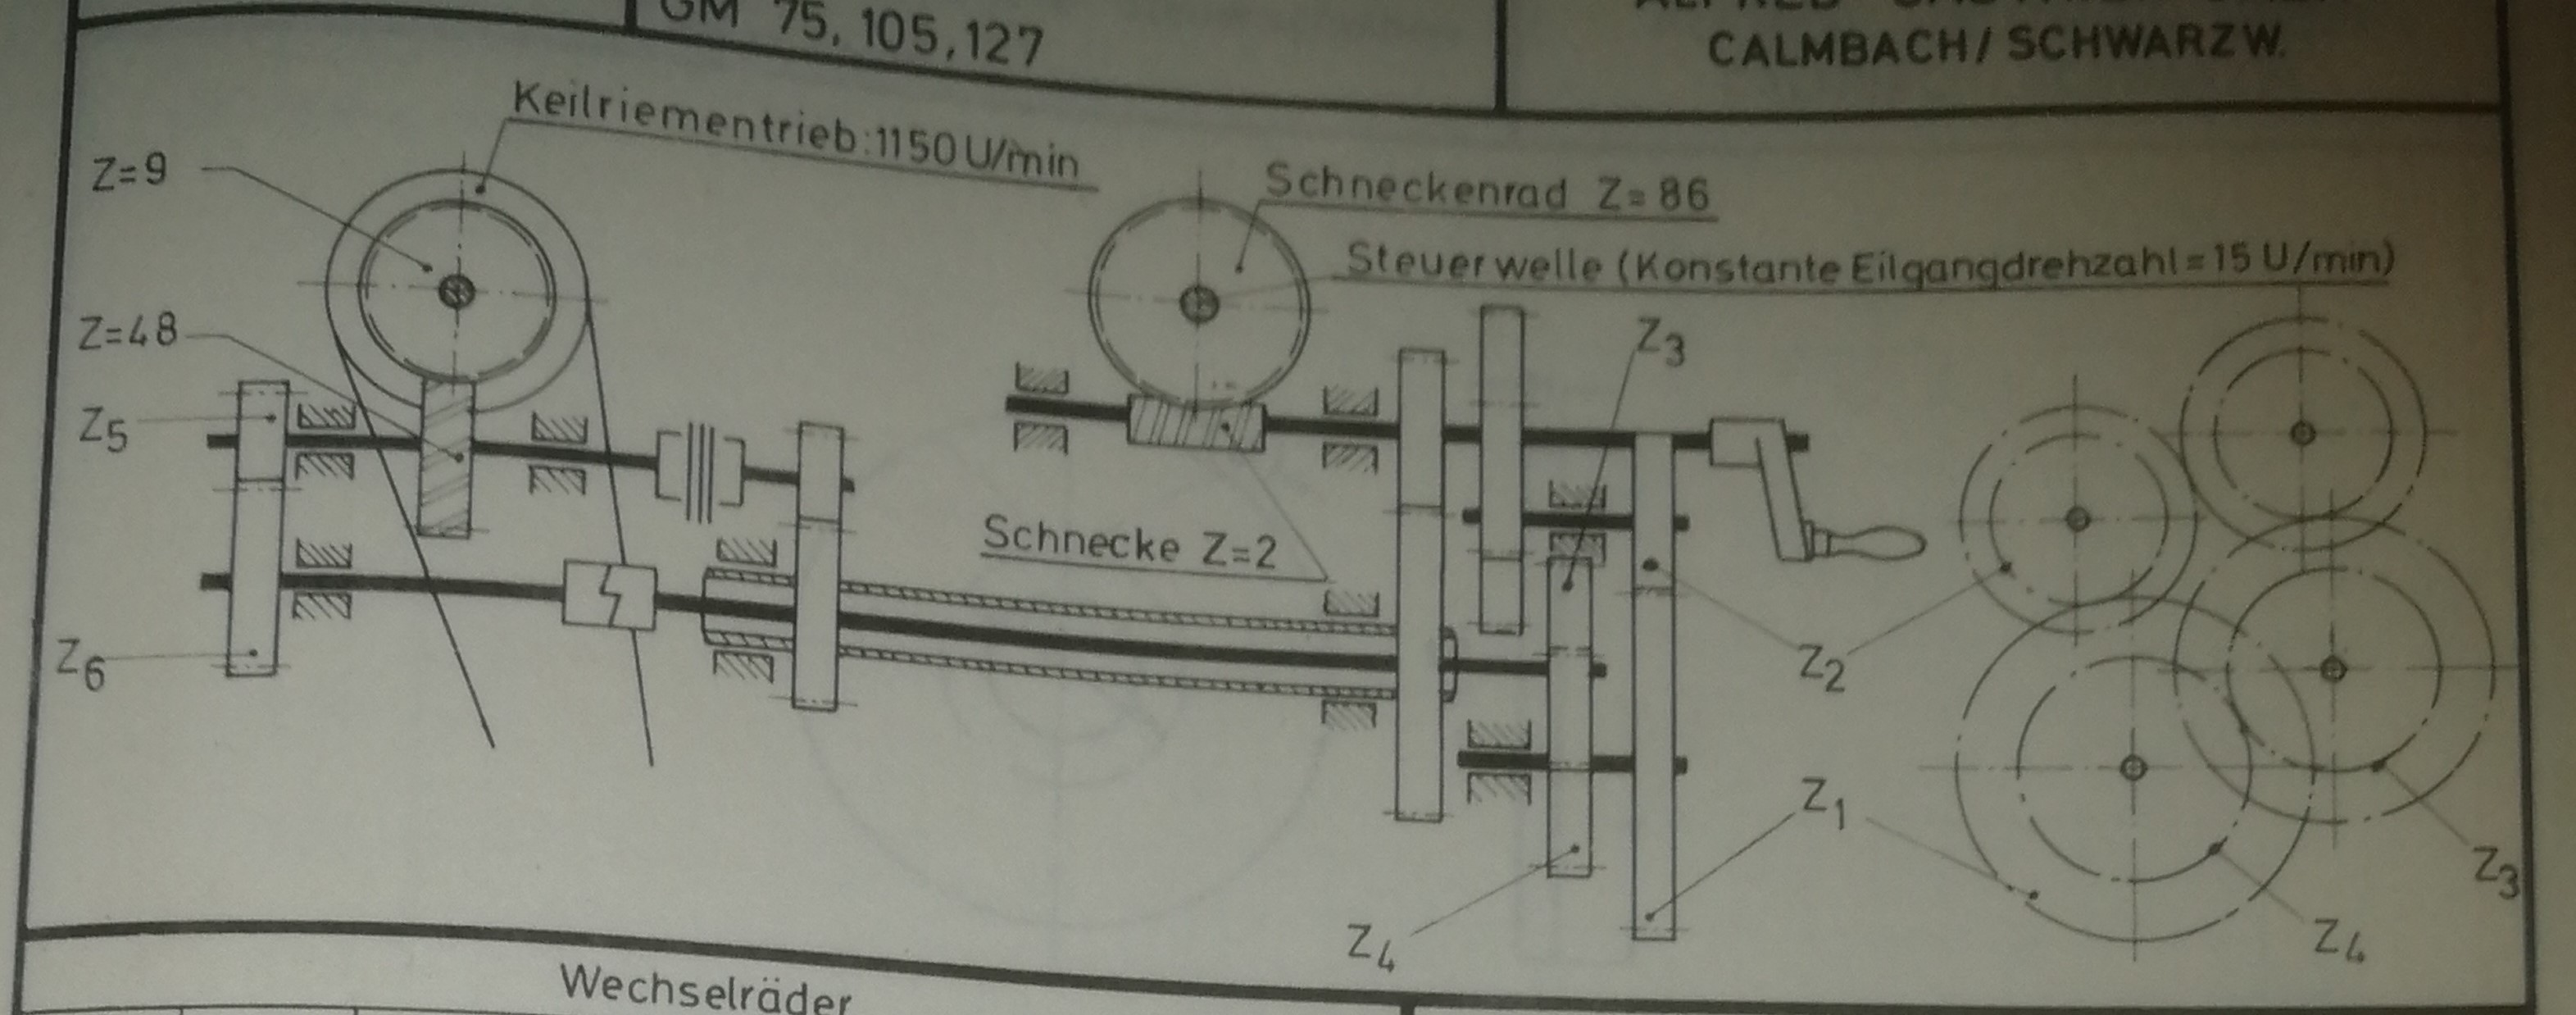
\includegraphics[width=\linewidth]{shema_tabela_krivuljna_gred.jpg}
		\caption{Povečava sheme jermenov in zobnikov
			hitrosti krivuljne gredi
			\cite{gauthier}}
		\label{povecava}
	\end{center}
\end{figure}

Potem določimo še vse potrebne zobnike tako, da jih razberemo iz tabele: \\
\(Z_1 = 45\ zob, Z_2 = 40\ zob, Z_3 = 25\ zob, Z_4 = 60\ zob, Z_5 = 70\ zob, Z_6 = 26\ zob\).
Ostali zobniki pa ostanejo enaki.

Zdaj, ko imamo vse krivulje in zobnike preračunane, nam preostane še montiranje izbranih
zobnikov, stročnic in orodja. Montaža zobnikov je dokaj enostavna.
Fiksirani so na osi s protiodvojno matico in segerjevim obročem,
ki ju odstranimo in enostavno zamenjamo zobnike. Menjava jermenov pa je veliko težja, saj je jermen napeljan okoli glavne osi,
ki jo je potrebno popolnoma razstaviti, kar traja dlje časa.